\begin{figure}
	\centering
	\begin{tikzpicture}[
		scale=0.6,
		every node/.style={scale=0.9}
	]

		% draw rectangles
		\draw[ultra thick] (0,0) rectangle (3,8);
		\draw[ultra thick] (4,0) rectangle (11,8);
		\draw[ultra thick] (12,0) rectangle (15,8);

		\node at (1.5,8.5) {\footnotesize{Apriori Probabilities}};
		\node at (7.5,8.5) {\footnotesize{Feature Contributions}};
		\node at (13.5,8.5) {\footnotesize{Aposteriori Probabilities}};

		\node at (3.5,4) {x};
		\node at (7.5,4) {x ... x};
		\node at (11.5,4) {=};
	
		% first coordinate system
		\node at (1.5,4) {
			\begin{tikzpicture}[scale=0.7]
				\node at (1.5,8) {\footnotesize{$p(\mathcal{C}_k)$}};
		
				\draw[fill=red!30,draw=red,thick] (0.8,3) rectangle (1.2,6.2);
				\draw[fill=blue!30,draw=blue,thick] (1.4,3) rectangle (1.8,5.8);
				\draw[fill=green!30,draw=green,thick] (2.0,3) rectangle (2.4,6.9);

				\draw[thick] (0.5,3) -- (2.5,3);
				\draw[thick] (0.5,3) -- (0.5,7);

				\node[rotate=90] at (1.0,2.0) {\footnotesize{Class 1}};
				\node[rotate=90] at (1.6,2.0) {\footnotesize{Class 2}};
				\node[rotate=90] at (2.2,2.0) {\footnotesize{Class 3}};
			\end{tikzpicture}
		};

		% second coordinate system
		\node at (5.5,4) {
			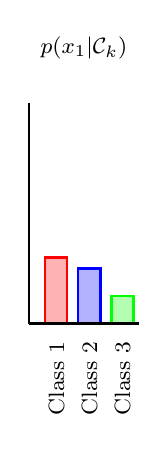
\begin{tikzpicture}[scale=0.7]
				\node at (1.5,8) {\footnotesize{$p(x_1 \vert \mathcal{C}_k)$}};

				\draw[fill=red!30,draw=red,thick] (0.8,3) rectangle (1.2,4.2);
				\draw[fill=blue!30,draw=blue,thick] (1.4,3) rectangle (1.8,4.0);
				\draw[fill=green!30,draw=green,thick] (2.0,3) rectangle (2.4,3.5);

				\draw[thick] (0.5,3) -- (2.5,3);
				\draw[thick] (0.5,3) -- (0.5,7);

				\node[rotate=90] at (1.0,2.0) {\footnotesize{Class 1}};
				\node[rotate=90] at (1.6,2.0) {\footnotesize{Class 2}};
				\node[rotate=90] at (2.2,2.0) {\footnotesize{Class 3}};
			\end{tikzpicture}
		};

		% third coordinate system
		\node at (9.5,4) {
			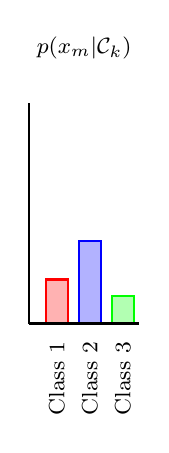
\begin{tikzpicture}[scale=0.7]
				\node at (1.5,8) {\footnotesize{$p(x_m \vert \mathcal{C}_k)$}};

				\draw[fill=red!30,draw=red,thick] (0.8,3) rectangle (1.2,3.8);
				\draw[fill=blue!30,draw=blue,thick] (1.4,3) rectangle (1.8,4.5);
				\draw[fill=green!30,draw=green,thick] (2.0,3) rectangle (2.4,3.5);

				\draw[thick] (0.5,3) -- (2.5,3);
				\draw[thick] (0.5,3) -- (0.5,7);

				\node[rotate=90] at (1.0,2.0) {\footnotesize{Class 1}};
				\node[rotate=90] at (1.6,2.0) {\footnotesize{Class 2}};
				\node[rotate=90] at (2.2,2.0) {\footnotesize{Class 3}};
			\end{tikzpicture}
		};

		% fourth coordinate system
		\node at (13.5,4) {
			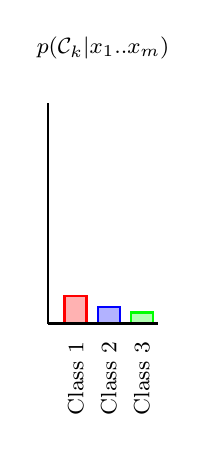
\begin{tikzpicture}[scale=0.7]
				\node at (1.5,8) {\footnotesize{$p(\mathcal{C}_k \vert x_1..x_m)$}};

				\draw[fill=red!30,draw=red,thick] (0.8,3) rectangle (1.2,3.5);
				\draw[fill=blue!30,draw=blue,thick] (1.4,3) rectangle (1.8,3.3);
				\draw[fill=green!30,draw=green,thick] (2.0,3) rectangle (2.4,3.2);

				\draw[thick] (0.5,3) -- (2.5,3);
				\draw[thick] (0.5,3) -- (0.5,7);

				\node[rotate=90] at (1.0,2.0) {\footnotesize{Class 1}};
				\node[rotate=90] at (1.6,2.0) {\footnotesize{Class 2}};
				\node[rotate=90] at (2.2,2.0) {\footnotesize{Class 3}};
			\end{tikzpicture}
		};

	\end{tikzpicture}
\end{figure}
